\chapter{Przegląd istniejących rozwiązań}
	Procesor Zilog Z80 dorobił się wielu emulatorów, pisanych kiedyś przez duże firmy, a aktualnie przez hobbystów. Na popularnej usłudze hostingowej Github przeznaczonej dla projektów programistycznych, można znaleźć około 200 repozytoriów z projektami emulującymi Z80, lub emulującymi urządzenia używające tego procesora, co dowodzi jego popularności.\cite{githubZ80Emulators}   
	
	 Poniżej prezentuje najciekawsze pozycje tych programów, które pozwalają na wgląd w  wewnętrzne stany procesora. Przedstawię zarówno komercyjne rozwiązania, jak i te pisane przez amatorów.
	
	\section{Z80 SIMULATOR IDE}
	Dostępny pod adresem http://www.oshonsoft.com/z80.html płatny symulator posiadający najbardziej rozbudowany interfejs z wszystkich wymienionych pozycji. Pozwala on na prezentowanie wewnętrznych stanów procesora, manipulacją przerwaniami, edytor pamięci umożliwiający działający również podczas symulacji, podgląd i manipulacja portami wejścia/wyjścia. Posiada również funkcje typowe dla debuggerów, możliwość wstrzymania działania programu w określonym miejscu, tryb pracy krokowej, interaktywny edytor i kompilator kodu asemblera.\cite{oshonsoftEmulator} Część funkcji została zaprezentowana na rysunku \ref{img:oshonsoftEmulator} 
	
	\begin{figure}[h]
		\centering
		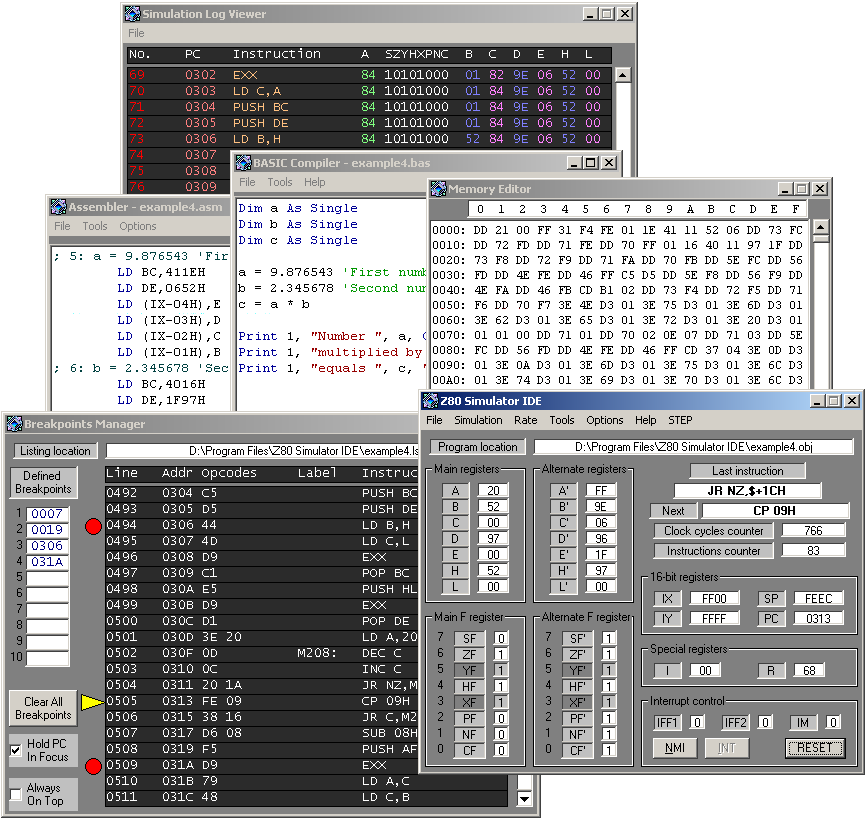
\includegraphics[width=0.7\textwidth]{oshonsoftEmulator}
		\caption{Z80 SIMULATOR IDE \cite{oshonsoftEmulator}}
		\label{img:oshonsoftEmulator}
	\end{figure}
	
	Do wad emulatora należy interfejs, który nie jest intuicyjny. Dla przykładu, w żadnym miejscu nie znajdziemy informacji, o tym w jakim formacie powinny być wprowadzane wartości liczbowe. Brak w programie systemu pomocy, opisów, co może odstraszyć początkującego użytkownika. Dodatkowo jest to rozwiązanie płatne i przeznaczone tylko dla platformy MS Windows. Jest to narzędzie głównie dla specjalistów.
	
	
	\section{ZEMU - Z80 Emulator Joe Moore}
	
	

	Żadne istniejące rozwiązanie nie pozwala na podejrzenie wewnętrznych magistrali procesora
	
	\section{Motywacja}
	dsadsadsa